% =====================================================================
%  Reporte.tex
%  ========================
%
%
%  Descripción:
%  ------------
%  Reporte de la actividad de correlación y regresión de Matemáticas
%  para la Computación, versión de Arturo Zabdi Reyes Pérez: modelo
%  lineal del precio de los anuncios de Airbnb en la Ciudad de México
%  con baños, posición este-oeste y tipo de alojamiento, en el corte
%  de septiembre de 2026. Clase LNCS de Springer, en tono formal.
%
%
%  Considerations:
%  ------------
%  - Compila con pdflatex y latexmk; llncs.cls viene en TeX Live
%  - Todas las cifras salen de Regresion.ipynb, y las figuras de
%    figuras/ las escribe el mismo notebook
%
%
%  Metadata:
%  ----------
%   * Author : zxxz6 (Bryan Violante Arriaga)
%   * Version: 1.0.0
%
%
%  History:
%  ------------
%  Author      Date            Description
%  zxxz6       13/11/2026      Creation
%
%
% =====================================================================
\documentclass{llncs}

\usepackage[letterpaper,margin=2.5cm]{geometry}
\usepackage[T1]{fontenc}
\usepackage[spanish,es-noshorthands,es-tabla,es-nodecimaldot]{babel}
\usepackage{graphicx}
\usepackage{booktabs}
\usepackage{amsmath}
\usepackage{array}
\usepackage[hidelinks]{hyperref}
\urlstyle{same}

\graphicspath{{figuras/}}

\renewcommand{\topfraction}{0.85}
\renewcommand{\textfraction}{0.1}
\renewcommand{\floatpagefraction}{0.8}

\newcolumntype{L}[1]{>{\raggedright\arraybackslash}p{#1}}

\begin{document}

\renewcommand{\figurename}{Fig.}
\renewcommand{\tablename}{Tabla}
\pagestyle{plain}

\noindent Arturo Zabdi Reyes Pérez \hfill Matemáticas para la
Computación\\
\phantom{x}\hfill 13 de noviembre de 2026
\medskip\hrule\bigskip

\bigskip

{\centering\Large\bfseries Actividad\par}

\bigskip


En esta actividad se analiza el precio por noche de los anuncios de
Airbnb en la Ciudad de México a partir del corte del 23 de septiembre de
2026 de Inside
Airbnb\footnote{\url{https://insideairbnb.com/get-the-data/}}, el mismo
conjunto de datos del proyecto. Se conservan los 28,289 anuncios con
precio entre 100 y 50,000 pesos y con número de baños registrado,
publicados por 12,205 anfitriones.

El modelo tiene un propósito explicativo y no predictivo: se busca
cuantificar la asociación entre el precio y un número reducido de
atributos, cada uno con los demás constantes. Esta decisión orienta el
resto del análisis, ya que exige predictores con baja correlación entre
sí, coeficientes interpretables y errores estándar confiables.

\bigskip

\noindent\textbf{Declaración de uso de IA:} En esta actividad se
utilizaron herramientas de inteligencia artificial como apoyo en el
análisis de los datos, la generación de gráficas y la elaboración del
código.


\section*{Selección de las variables}

Se consideraron trece variables candidatas: características físicas
del inmueble (recámaras, camas, baños y número de amenidades), ubicación
geográfica (latitud y longitud), tipo de alojamiento (indicadora de
alojamiento entero frente a cuarto), condición de superanfitrión,
número de reseñas, días disponibles al año, noches mínimas, número de
anuncios del anfitrión y antigüedad del anfitrión en la plataforma. Se
calculó la correlación de Spearman entre todos los pares
(Fig.~\ref{fig:correlacion}), por ser robusta ante las colas largas
que presentan varias de estas variables.

\begin{figure}[h!]
\centering
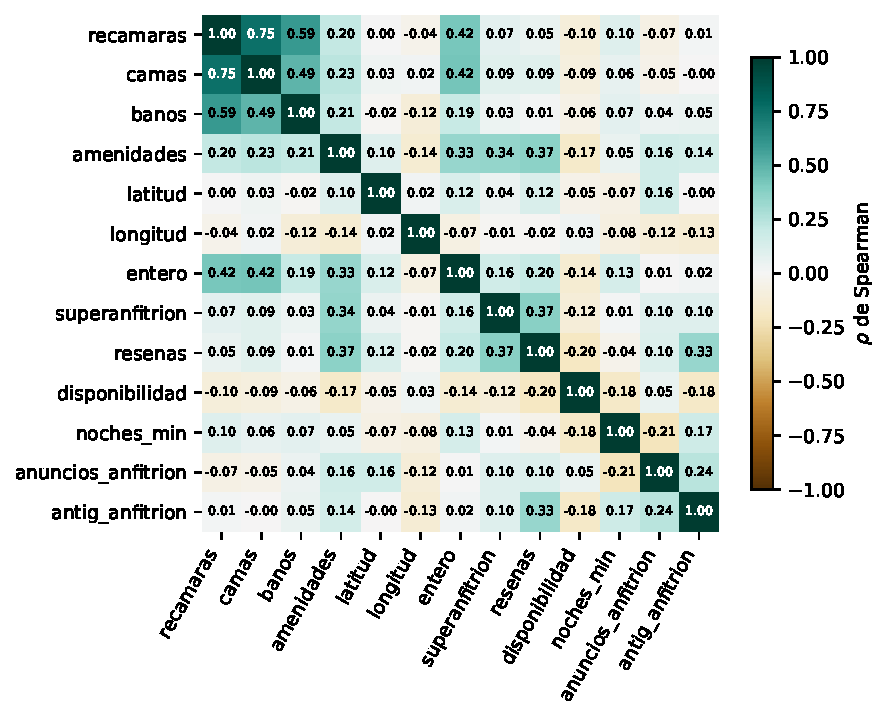
\includegraphics[width=0.6\textwidth]{Correlacion.pdf}
\caption{Matriz de correlación de Spearman entre las trece variables
candidatas ($n = 28{,}323$).}
\label{fig:correlacion}
\end{figure}

\newpage

Recámaras, camas y baños forman un bloque de alta correlación (0.49 a
0.75), pues las tres miden el tamaño del inmueble. Fuera de ese bloque
se observan correlaciones moderadas, entre 0.33 y 0.42, del
alojamiento entero con recámaras, camas y amenidades, y de las
amenidades, las reseñas y la condición de superanfitrión entre sí.

Para la selección se evaluaron las 286 ternas posibles. Se
consideraron admisibles las 190 en las que todos los pares cumplen
$|\rho| < 0.3$, y entre ellas se eligió la de mayor asociación conjunta
con el logaritmo del precio. La terna seleccionada es
\textbf{baños, longitud y alojamiento entero}, con una correlación
máxima de 0.19 entre sus pares y factores de inflación de la varianza
de 1.01 en las tres variables. Cada una representa una dimensión
distinta del anuncio: tamaño, ubicación y tipo de alojamiento. Para
facilitar la interpretación, la longitud se expresa como distancia en
kilómetros al este del meridiano del Ángel de la Independencia; al ser
una transformación lineal, no modifica ninguna correlación.


\section*{Análisis exploratorio}

\begin{figure}[h]
\centering
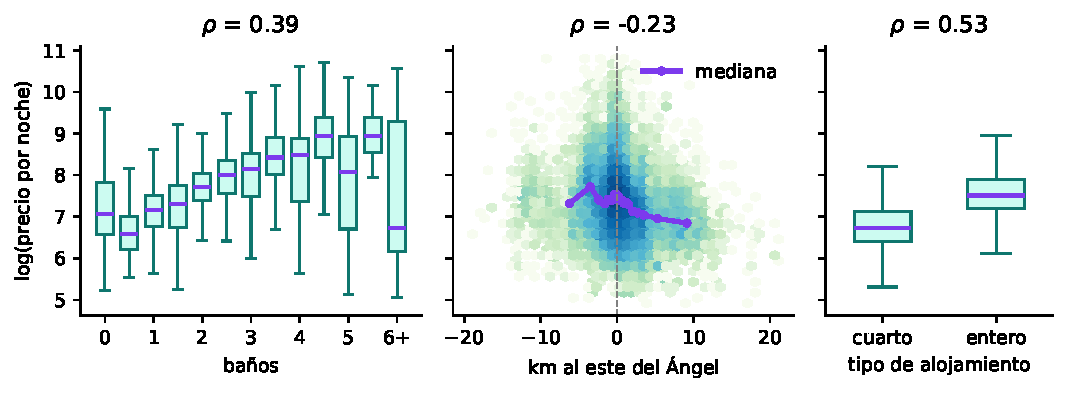
\includegraphics[width=\textwidth]{Dispersion.pdf}
\caption{Logaritmo del precio contra cada predictor. Las cajas omiten
los valores atípicos; en el panel central, la línea es la mediana por
veintil y la línea punteada marca el meridiano del Ángel.}
\label{fig:dispersion}
\end{figure}

La Fig.~\ref{fig:dispersion} muestra tres relaciones de forma distinta.
El precio crece con el número de baños hasta alrededor de cinco, pero a
partir de seis la dispersión aumenta y la mediana desciende, porque en
ese grupo se concentran hostales con baños compartidos. En la dirección
este-oeste, el precio alcanza su máximo ligeramente al poniente del
Ángel y desciende hacia el oriente. El alojamiento entero tiene un
precio mediano de 1,827 pesos, frente a 841 pesos de un cuarto.


\section*{Especificación y ajuste del modelo}

El primer modelo relaciona linealmente el precio con las tres
variables y se ajusta por mínimos cuadrados ordinarios. Su ajuste es
pobre ($R^2 = 0.18$) y sus residuos presentan una asimetría de 7.1 y
una curtosis de 94, producto de unos cuantos anuncios de precio muy
alto que dominan la suma de cuadrados. Al tomar el logaritmo del precio
el $R^2$ sube a 0.33 y los residuos se vuelven aproximadamente
simétricos. El análisis de residuos por clase mostró, además, que los
anuncios con seis o más baños aplanaban la pendiente del número de
baños, por lo que esta variable se sustituyó por
$\log(1 + \text{baños})$, que reduce la influencia de los valores
extremos y admite anuncios sin baño. La Tabla~\ref{tab:modelos} resume
los tres modelos y el modelo final es
\begin{equation}
\log(\text{precio}) = \beta_0 + \beta_1 \log(1 + \text{baños})
+ \beta_2\,\text{este} + \beta_3\,\text{entero} + \varepsilon ,
\label{eq:final}
\end{equation}
donde \emph{este} es la distancia en kilómetros al este del meridiano
del Ángel y \emph{entero} vale 1 para un alojamiento entero y 0 para
un cuarto.

\begin{table}[h]
\caption{Comparación de los modelos ajustados. El RMSE del modelo 0
está en pesos y el de los demás en escala logarítmica; BP es el
estadístico de Breusch-Pagan, con valor $p$ prácticamente nulo en los
tres casos.}
\label{tab:modelos}
\centering
\begin{tabular}{@{}lccccc@{}}
\toprule
Modelo & $R^2$ & RMSE & Asimetría & Curtosis & BP \\
\midrule
0: precio & 0.181 & 2,330 & 7.10 & 93.8 & 1,124 \\
1: $\log(\text{precio})$ & 0.328 & 0.605 & 0.46 & 3.98 & 4,158 \\
2: con $\log(1 + \text{baños})$ & 0.347 & 0.596 & 0.60 & 2.96 & 1,584 \\
\bottomrule
\end{tabular}
\end{table}

Los errores estándar se calcularon de forma robusta y agrupada por
anfitrión, ya que los anuncios de un mismo anfitrión no son
observaciones independientes. La diferencia es considerable: para el
coeficiente de los baños, el error agrupado es seis veces mayor que el
clásico, debido a los anfitriones que publican muchos anuncios
similares. Los tres coeficientes son significativos con $p < 0.001$
(Tabla~\ref{tab:coeficientes}).

\begin{table}[h]
\caption{Coeficientes del modelo final \eqref{eq:final}, con error
estándar robusto agrupado por anfitrión e intervalo de confianza de
95\,\%.}
\label{tab:coeficientes}
\centering
\begin{tabular}{@{}lcccL{5.6cm}@{}}
\toprule
Término & $\hat\beta$ & EE & IC 95\,\% & Interpretación \\
\midrule
Intercepto & 6.252 & 0.054 & [6.146, 6.358] & Cuarto sin baño en el
meridiano del Ángel \\
$\log(1 + \text{baños})$ & 0.752 & 0.076 & [0.602, 0.902] & Pasar de
1 a 2 baños se asocia con un precio 35.6\,\% mayor \\
Este (km) & $-0.031$ & 0.003 & [$-0.036$, $-0.026$] & Cada kilómetro
hacia el oriente reduce el precio 3.1\,\% \\
Entero & 0.684 & 0.025 & [0.634, 0.733] & Un alojamiento entero cuesta
98\,\% más que un cuarto \\
\bottomrule
\end{tabular}
\end{table}


\section*{Diagnóstico}

\begin{figure}[h]
\centering
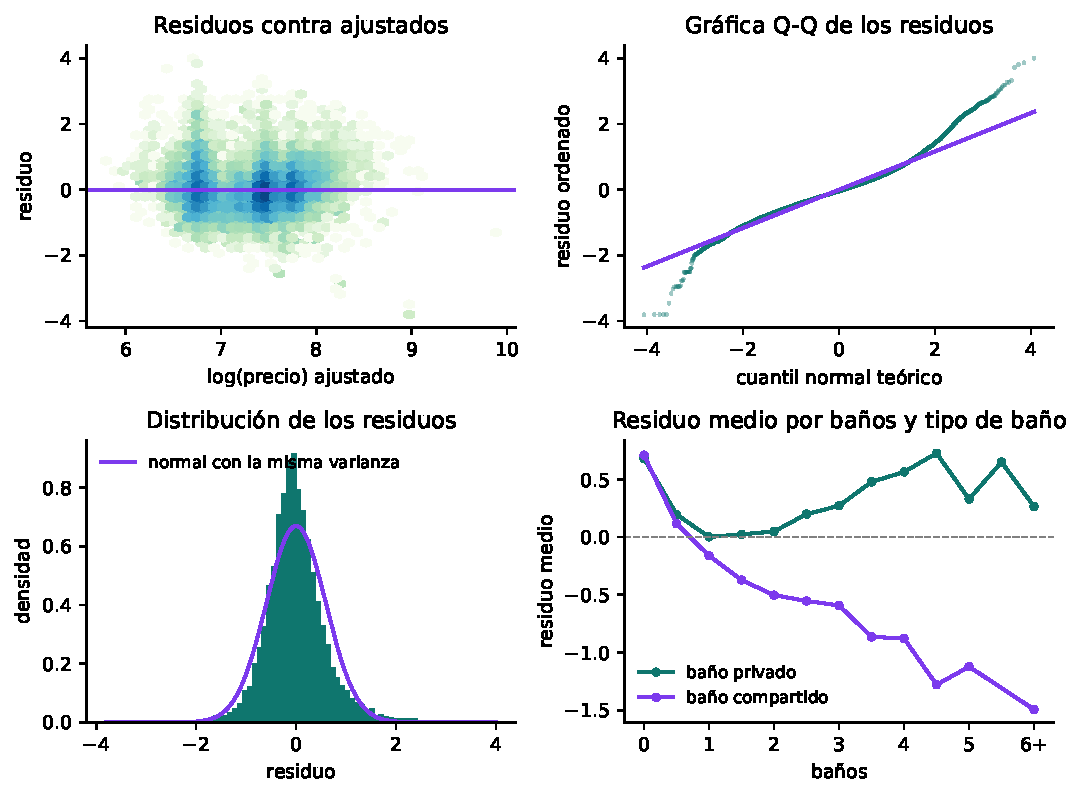
\includegraphics[width=0.8\textwidth]{Diagnostico.pdf}
\caption{Diagnóstico del modelo final. El último panel muestra el
residuo medio por número de baños, por separado para baños privados y
compartidos.}
\label{fig:diagnostico}
\end{figure}

Los residuos del modelo final (Fig.~\ref{fig:diagnostico}) se
distribuyen alrededor de cero sin tendencia respecto a los valores
ajustados; las bandas verticales se deben al carácter discreto de dos
de los predictores. La gráfica Q-Q indica colas más pesadas que las de
una distribución normal en ambos extremos. La prueba de Breusch-Pagan
rechaza la homocedasticidad: la desviación estándar residual es de 0.71
en cuartos y de 0.53 en alojamientos enteros, lo que justifica el uso
de errores estándar robustos.

El hallazgo principal del diagnóstico aparece en el último panel. Con
baño privado, el residuo crece con el número de baños; con baño
compartido, decrece. El número de baños agrupa dos poblaciones con
pendientes opuestas: en un inmueble privado, más baños indican un
inmueble más grande y caro, mientras que en un hostal indican más
camas en dormitorios compartidos y un precio menor. El modelo promedia
ambas tendencias. Incorporar una indicadora de baño compartido elevaría
el $R^2$ a 0.38, pero introduciría una cuarta variable correlacionada
con el tipo de alojamiento. De forma análoga, los 755 anuncios
situados a más de 6\,km al poniente, principalmente en Cuajimalpa y
Álvaro Obregón, resultan más baratos de lo que predice el término
lineal; un término cuadrático en la posición este-oeste corrige este
efecto, pero aporta menos de una centésima al $R^2$.

Para verificar la estabilidad del ajuste se reservó el 20\,\% de los
anuncios como partición de prueba. El $R^2$ en prueba es de 0.343,
frente a 0.348 en entrenamiento, y los coeficientes estimados varían
solo en el tercer decimal, por lo que no hay evidencia de
sobreajuste. Como herramienta de predicción el modelo es limitado: el
error absoluto mediano en prueba es de 449 pesos, equivalente al
32\,\% del precio.


\section*{Interpretación}

Al estar la respuesta en escala logarítmica, los efectos se expresan
como cambios porcentuales. El tipo de alojamiento es el factor de
mayor peso: con el mismo número de baños y la misma posición, un
alojamiento entero cuesta aproximadamente el doble que un cuarto. Pasar
de uno a tres baños se asocia con un aumento de 68\,\%, y desplazarse
5\,km hacia el oriente, con una reducción de 14\,\%. A modo de
referencia, el modelo estima un precio mediano de 1,732 pesos para un
alojamiento entero con un baño sobre el meridiano del Ángel, y de 874
pesos para un cuarto con las mismas características.


\section*{Limitaciones}

\begin{itemize}
\item El estudio es observacional; los coeficientes describen
asociaciones y no efectos causales.
\item El número de baños mezcla baños privados y compartidos, con
relaciones opuestas con el precio.
\item La posición este-oeste no captura la variación norte-sur ni las
diferencias entre colonias vecinas.
\item El precio corresponde al anunciado para las fechas cotizadas en
un único corte, no al pagado por los huéspedes.
\end{itemize}


\section*{Conclusiones}

Con tres variables poco correlacionadas, el modelo explica el 35\,\%
de la variación del logaritmo del precio. El tipo de alojamiento es el
determinante principal, seguido del número de baños y de la posición
este-oeste. El diagnóstico de residuos identificó con precisión la
principal deficiencia del modelo, la mezcla de baños privados y
compartidos, que constituye la mejora más directa para una
especificación posterior.

\end{document}

%############################# END OF REPORTE.TEX ##############################
%###############################################################################
